\subsection{Revisions and Commits}

Both Revision in Subversion and Commit in Git are atomic changes fixed at certain moment in time by certain person with certain message. The translation of this metadata described below.

\subsubsection{From Revision to Commit}

This kind of translation depicted at diagram \ref{single_change_svn_to_git}.

\begin{figure}[!h]
\centering
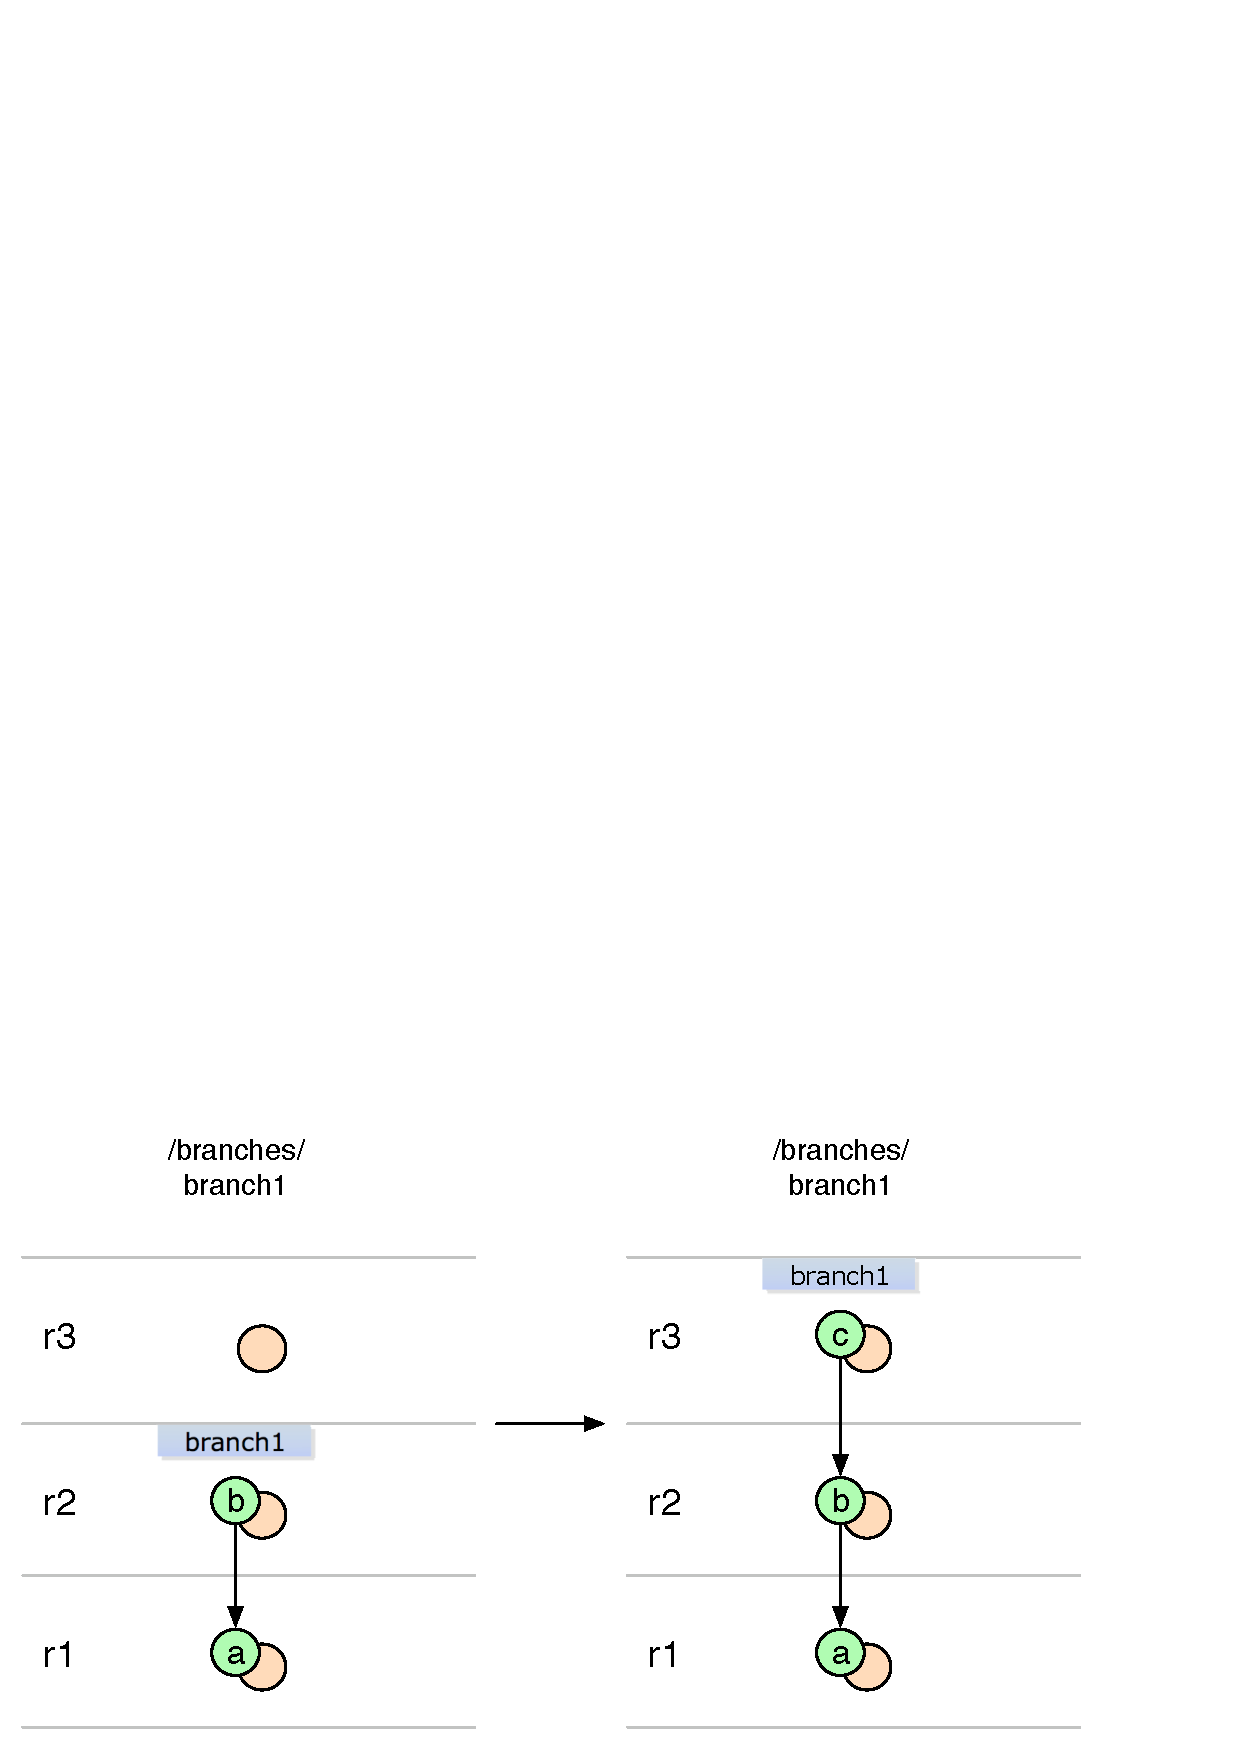
\includegraphics[width=\linewidth]{img/diagrams/single_change_svn_to_git.pdf}
\caption{Subversion revision being translated to Git commit creation.}
\label{single_change_svn_to_git}
\end{figure}

Subversion user modified /branches/branch1 at revision r3. For that change Translator
\begin{enumerate}
	\item Creates commit \emph{c} with Tree Object corresponding to /branches/branch1@r3 subdirectory contents.
	\item Commit \emph{c} has Author Ident and Committer Ident corresponding to the author of the revision.
	\item Commit \emph{c} has the same date as revision r3.
	\item Commit \emph{c} has the same message as the revision r3.
	\item Commit \emph{c} has Parent Commit \emph{b} which corresponds to revision r2, i.e. previous modification of branch1.
	\item And finally Translator updates reference /refs/heads/branch2 to the created commit \emph{c}.
\end{enumerate}

\subsubsection{From Commit to Revision}

This kind of translation depicted at diagram \ref{single_change_git_to_svn}.

\begin{figure}[!h]
\centering
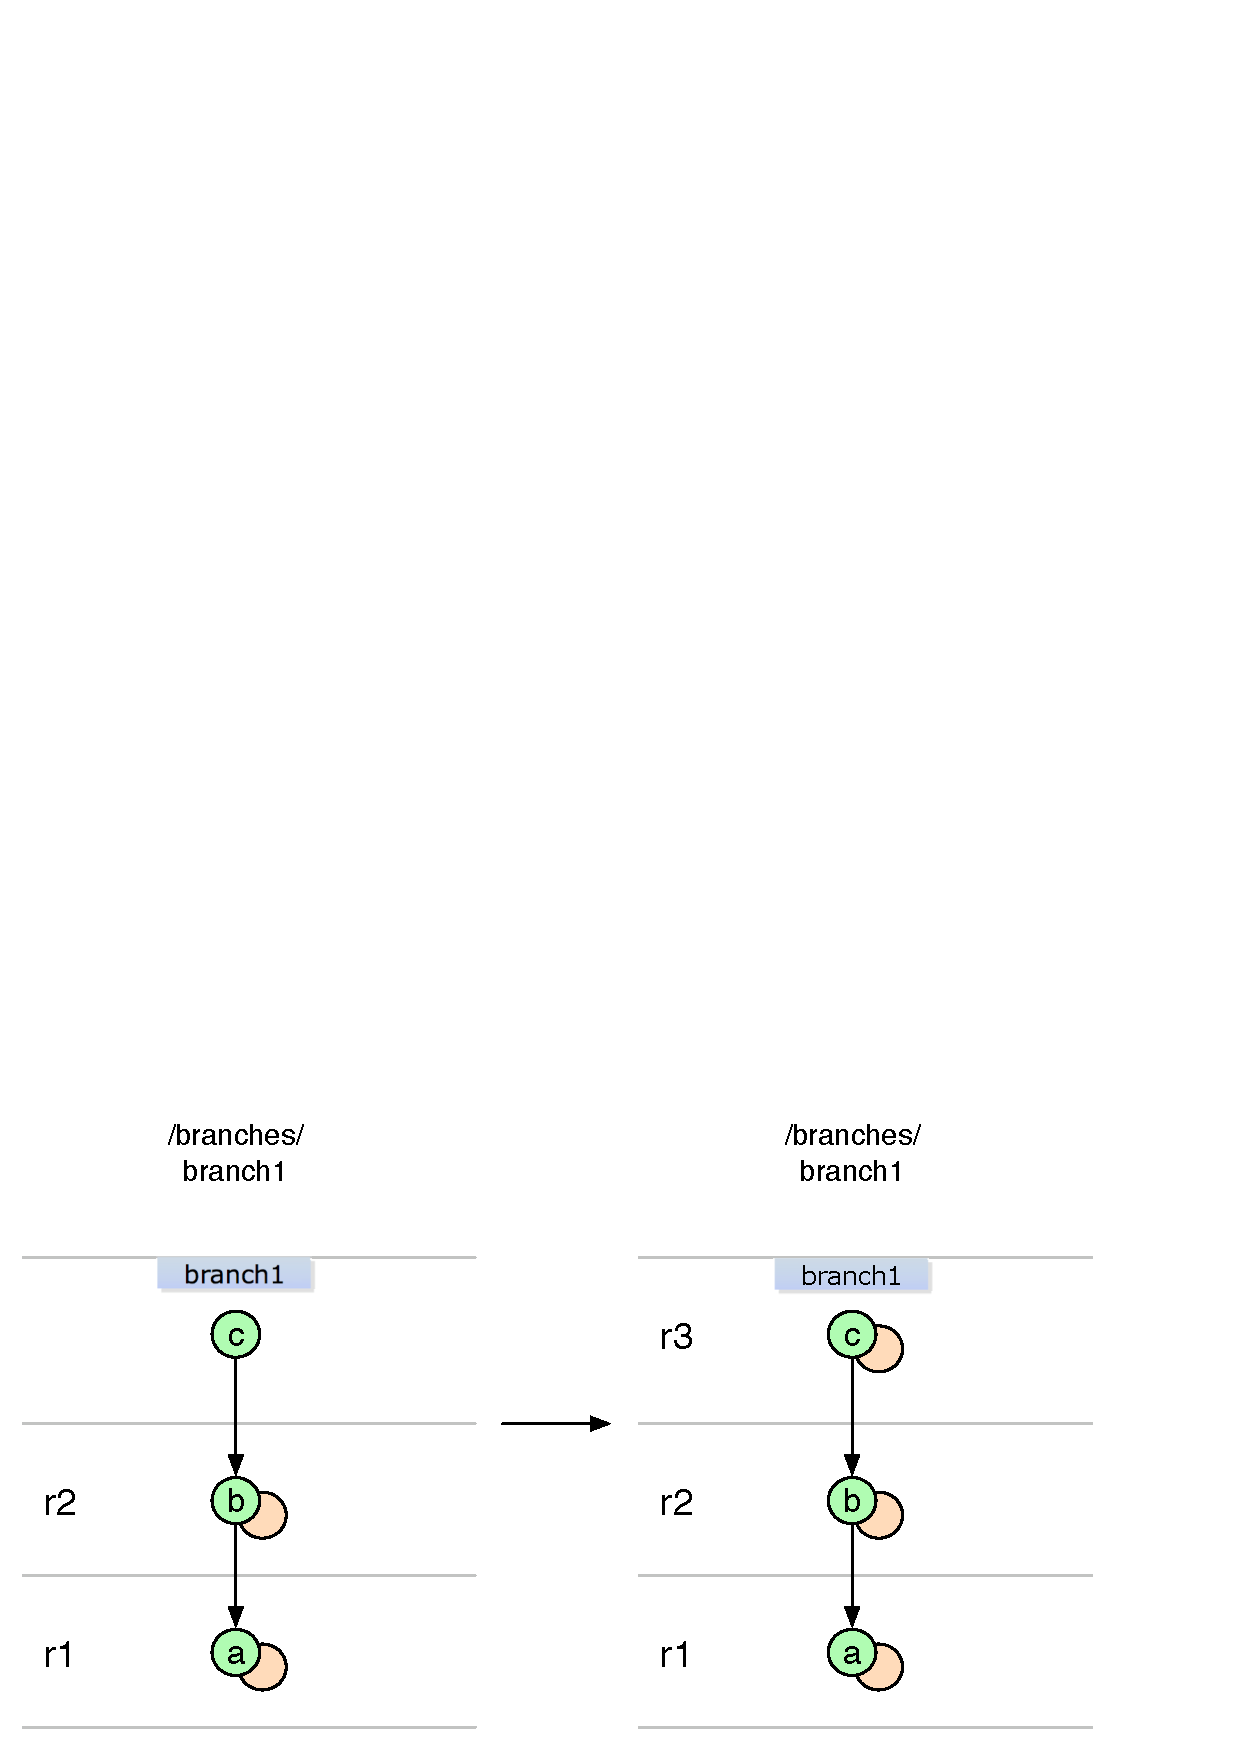
\includegraphics[width=\linewidth]{img/diagrams/single_change_git_to_svn.pdf}
\caption{Git Commit being translated to Subversion Revision.}
\label{single_change_git_to_svn}
\end{figure}

More complicated scenarios will be considered in the future chapters but metadata translation is common for any of them.